
\section{Rückblick}

\begin{frame}
  {Rückblick: Graphematik und Phonologie}
  \pause
  \begin{itemize}[<+->]
    \item Argumente, dass Graphematik zur Linguistik gehört
      \Halbzeile
    \item Schreibprinzipien
      \begin{itemize}[<+->]
        \item phonologisches Prinzip
        \item Gelenkschreibung
        \item offen geblieben: Warum \textit{Kinn}, \textit{Schutt} usw.?
        \item Eszett und die Eliminierung von /s/
      \end{itemize}
  \end{itemize}
\end{frame}


\section{Überblick}

\begin{frame}
  {Graphematik: Morphosyntaktisch motivierte Schreibungen}
  \pause
  Mehr Schreiprinzipien\\
  \Halbzeile
  \pause
  \begin{itemize}[<+->]
    \item Spatienschreibung
    \item Substantivgroßschreibung als positionsunabhängige Majuskelschreibung
    \item Konstantschreibung
      \Halbzeile
    \item dann nochmal Zusammenfassung aller Prinzipien
  \end{itemize}
  \pause
  \Halbzeile
  Danach (vor der Klausurbesprechung) noch zwei Ermahnungen\\
  \Halbzeile
  \pause
  \begin{itemize}[<+->]
    \item Nochmal zur Frage, was so schlimm daran ist, wenn \\
      traditionelle Lehrmethoden dem Problem nicht gerecht werden.
    \item Wo sprachliche Diskriminierung anfängt und\\
     warum Lehrer*innen als allerletzte sprachlich diskriminieren sollten.
  \end{itemize}
\end{frame}

\section{Wörter -- Spatien}

\begin{frame}
  {Boustrophedon: Gesetze von Gortys}
  \pause
  \centering
  \includegraphics[width=0.8\textwidth]{\GRAPHPATH/gortys}\\
  {\tiny (Kreta; griechisch (dorisch), 6.--5.\ Jh.\ u.\,Zr.)}
\end{frame}

\begin{frame}
  {Scriptio continua: Genji no Monogatari}
  \pause
  \centering
  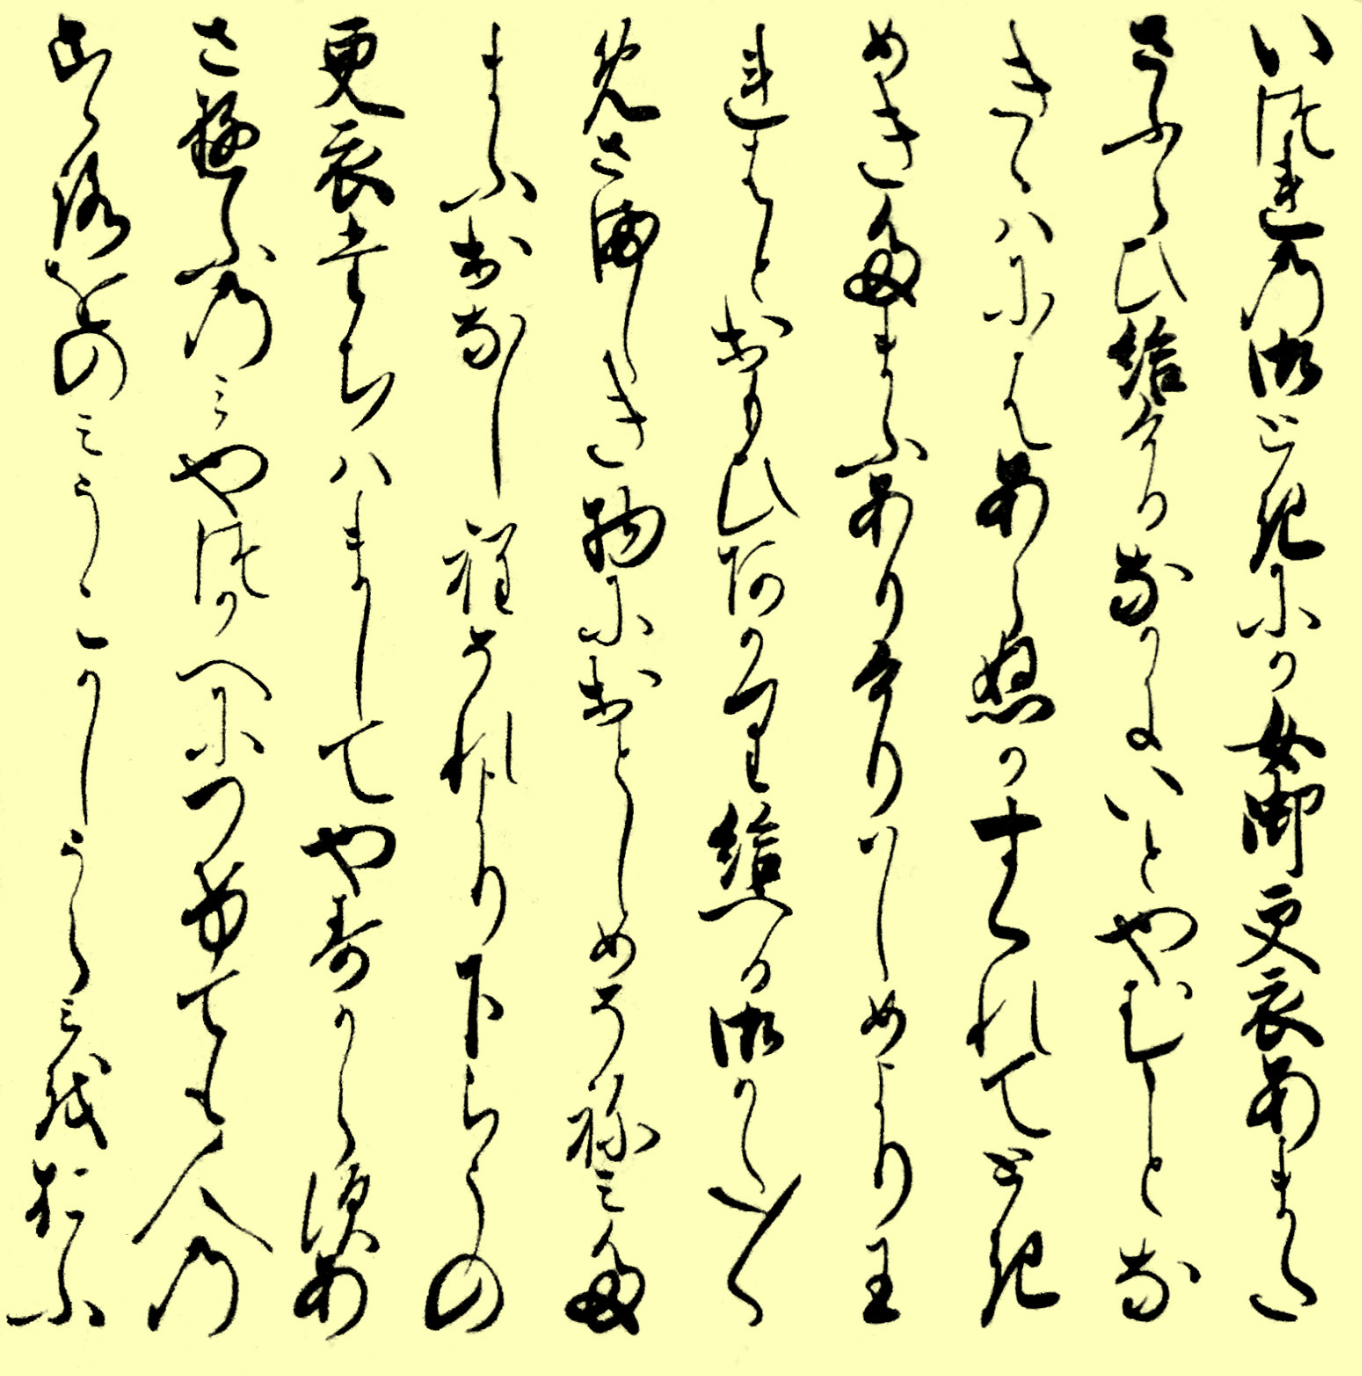
\includegraphics[width=0.55\textwidth]{\GRAPHPATH/genji1}\\
  {\tiny (\citealt{Rickmeyer1991}; 源氏物語:きりつぼ, ca. 1000 u.\,Zr., Manuskript (青表紙証本) ca.\ 1200 u.\,Zr.}
\end{frame}

\begin{frame}
  {Scriptio continua: Genji no Monogatari}
  \centering
  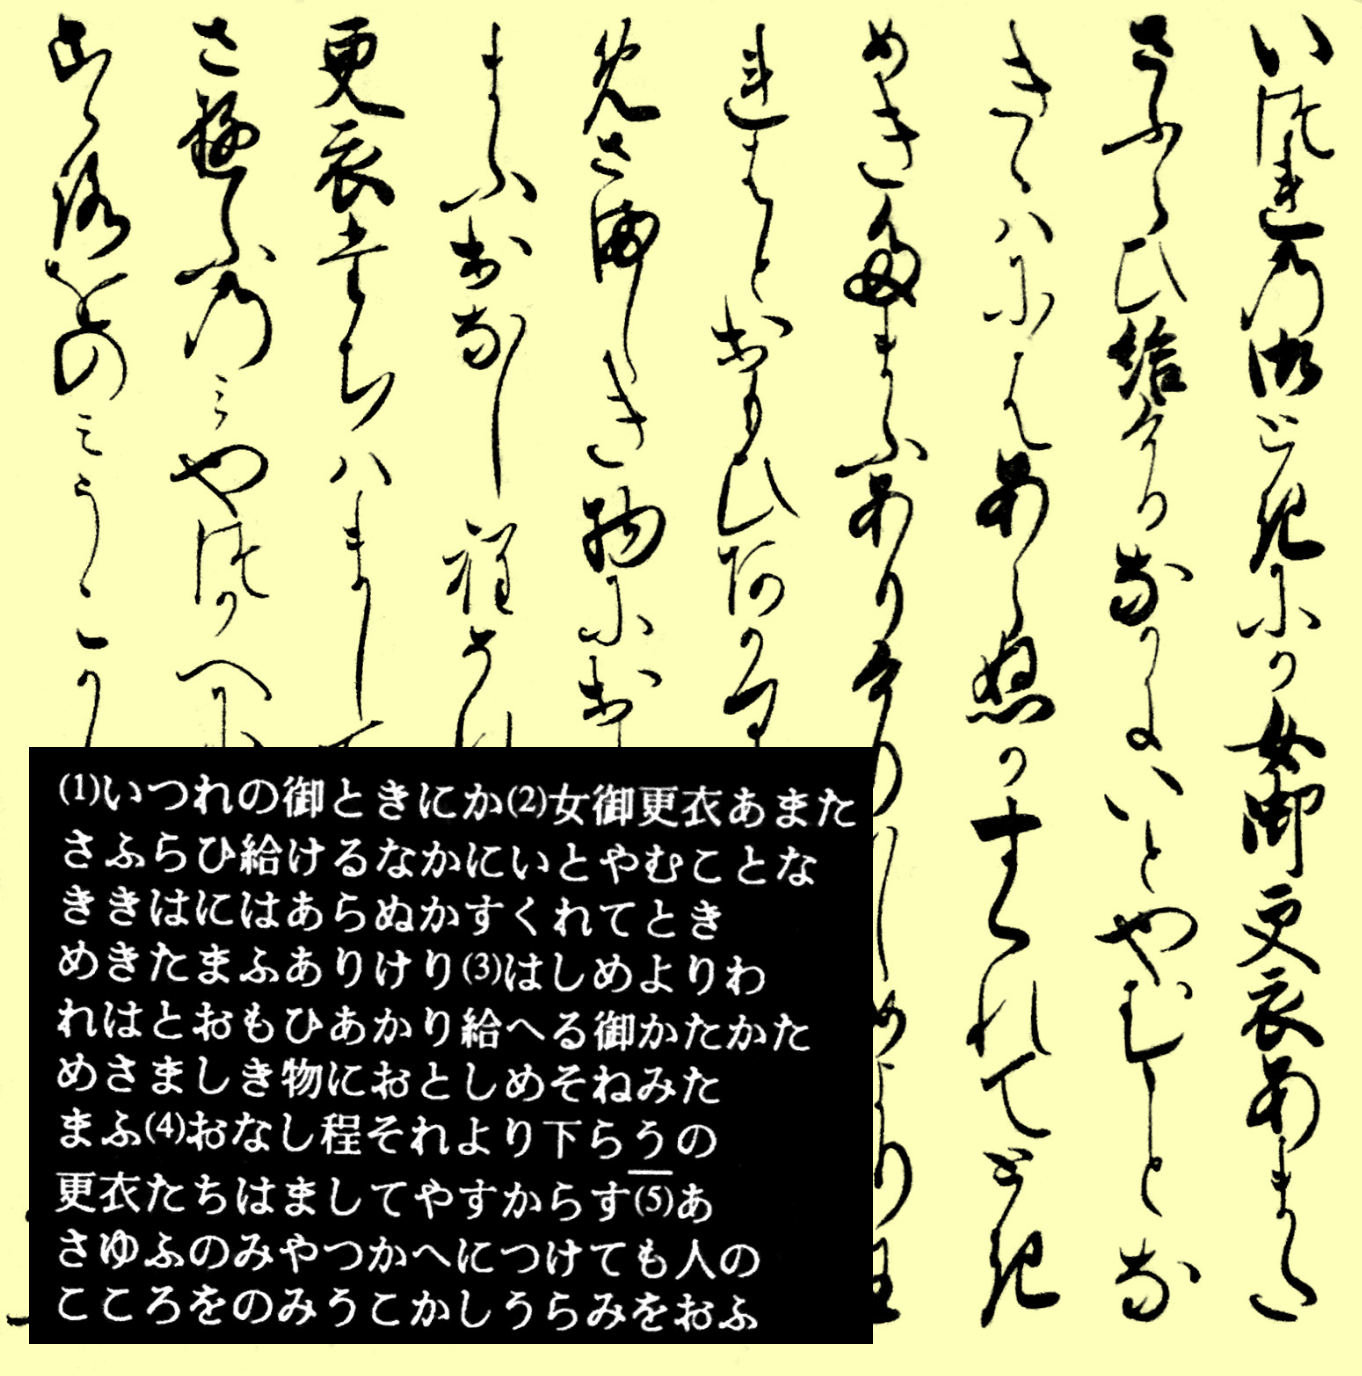
\includegraphics[width=0.55\textwidth]{\GRAPHPATH/genji3}\\
  {\tiny (\citealt{Rickmeyer1991}; 源氏物語:きりつぼ, ca. 1000 u.\,Zr., Manuskript (青表紙証本) ca.\ 1200 u.\,Zr.}
\end{frame}

\begin{frame}
  {Wie selbstverständlich ist unsere Schreibung?}
  \pause
  \centering
  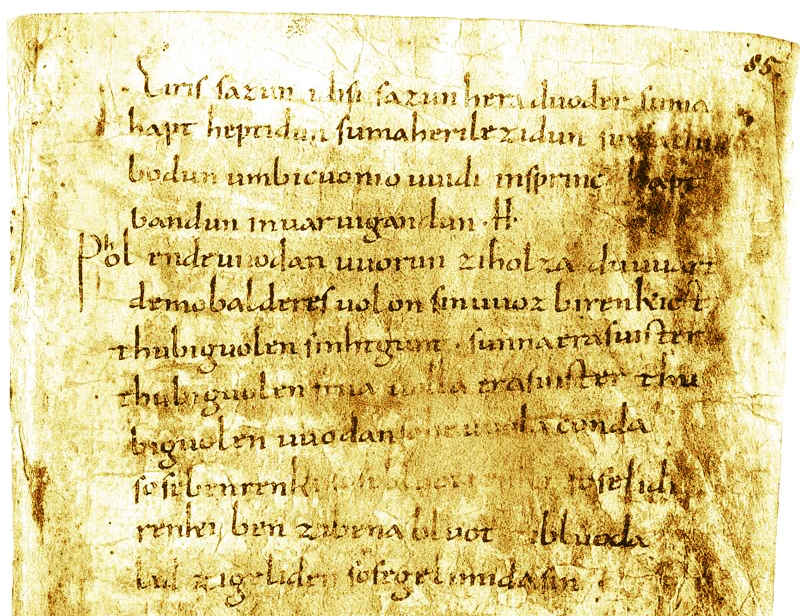
\includegraphics[width=0.8\textwidth]{\GRAPHPATH/merseburg}\\[0.5\baselineskip]
  {\tiny 1.~und 2.~Merseburger Zauberspruch, 9.~Jh.\ u.\,Zr., Cod.\ 136, Folio 85r, Domstiftsbibliothek Merseburg (Wikimedia)\\[-1\baselineskip]
    Hintergründe und generelle Einführung in historische Graphematik in \citet{Elmentaler2018}.}
\end{frame}

\begin{frame}
  {Spatien}
  \pause
  \begin{itemize}[<+->]
    \item im Ahd.\ häufig Reste von Scriptio continua
    \item syntaktische Wörter nicht immer getrennt
    \item \alert{Spatienschreibung}: Trennung syntaktischer Wörter
  \end{itemize}
  \pause
  \Halbzeile
  \begin{exe}
    \ex
    \begin{xlist}
      \ex[*]{Vanessa \rot{istgeritten}.}
      \pause
      \ex[*]{Vanessa reitet \rot{indenwald}.}
    \end{xlist}
    \pause
    \Halbzeile
    \ex
    \begin{xlist}
      \ex[*]{Vanessa hat \rot{Gelegen heit}, die \rot{Schreib ung} von Wörtern und Sätzen \rot{gründ lich} zu \rot{unter suchen}.}
      \pause
      \ex[*]{Oma \rot{koch t} der \rot{ausgekühlt en} Vanessa \rot{ein en heiß en} Tee.}
    \end{xlist}
  \end{exe}
  \pause
  \begin{itemize}[<+->]
    \item Eislaufen, Bergsteigen, Mutmachen, Teetrinken (?)
    \item weichklopfen, schlechtreden (?)
    \item nichtöffentlich, nichtprivat (?)
    \item zulasten (?)
  \end{itemize}
\end{frame}

\section[PUMS vs.\ PAMS]{Positionsunabhängige Majuskelschreibung}

\begin{frame}
  {Majuskelschreibungen}
  \pause
  \begin{itemize}[<+->]
    \item \alert{positionsabhängig}: Satzanfang (Syntax)
      \Halbzeile
    \item \alert{positionsunabhängig}: Substantive (Morphologie\slash Lexik)
    \item Positionsunabhängige Majuskelschreibung (PUMS)
      \Halbzeile
    \item Bredel: "`NP-Kopf-Großschreibung"' (= positions\rot{abhängig}, PAMS)
      \begin{itemize}[<+->]
        \item nein, weil auch in Listen, Überschriften usw.
        \item außerdem: dann Annahme SubstP als verschieden von PronP!\\
          \grau{Oder werden Pronomina als NP-Köpfe großgeschrieben?}
        \item jede Rettungsargumentation des PAMS-Ansatzes wird zirkulär 
        \item \ldots oder \alert{motiviert} die PUMS statt sie zu beschreiben
        \item \grau{Siehe Schäfer \& Sayatz (in Vorb.).}
      \end{itemize}
  \end{itemize}
\end{frame}


\begin{frame}
  {Propblemfälle für PUMS}
  \pause
  \begin{exe}
    \ex
    \begin{xlist}
      \ex{An der Nacht auf dem Land schätze ich vor allem \alert{das Dunkle}.}
      \pause
      \ex{Alle Pferde müssen geputzt werden. Vanessa putzt \alert{das schwarze}.}
      \pause
      \ex{Vanessa trägt in der Oper \alert{das Schwarze}.}
    \end{xlist}
    \Viertelzeile
    \pause
    \ex
    \begin{xlist}
      \ex[ ]{im \alert{übrigen}}
      \pause
      \ex[*]{im literarischen \rot{Übrigen}}
      \pause
      \ex[*]{Im \rot{Übrigen}\slash In dem \rot{Übrigen}, von dem wir gestern schon gesprochen haben, ist dieses Buch langweilig.}
    \end{xlist}
    \pause
    \Viertelzeile
    \ex
    \begin{xlist}
      \ex[*]{Edgar gab dem Kunden fachmännisches Recht.}
      \pause
      \ex[*]{Edgar setzte den Cadillac in einwandfreien Stand.}
    \end{xlist}
  \end{exe}
  \pause
  \begin{itemize}[<+->]
    \item Konversion
    \item Ellipse
    \item Ellipse plus Lexikalisierung
      \Halbzeile
    \item mögliches Testkriterium bei \alert{Univerbierung}: Modifikation
  \end{itemize}
\end{frame}

\section[Konstanz]{Konstantschreibung}

\begin{frame}
  {Die Entwicklung von Schreibprinzipien}
  \pause
  \centering
  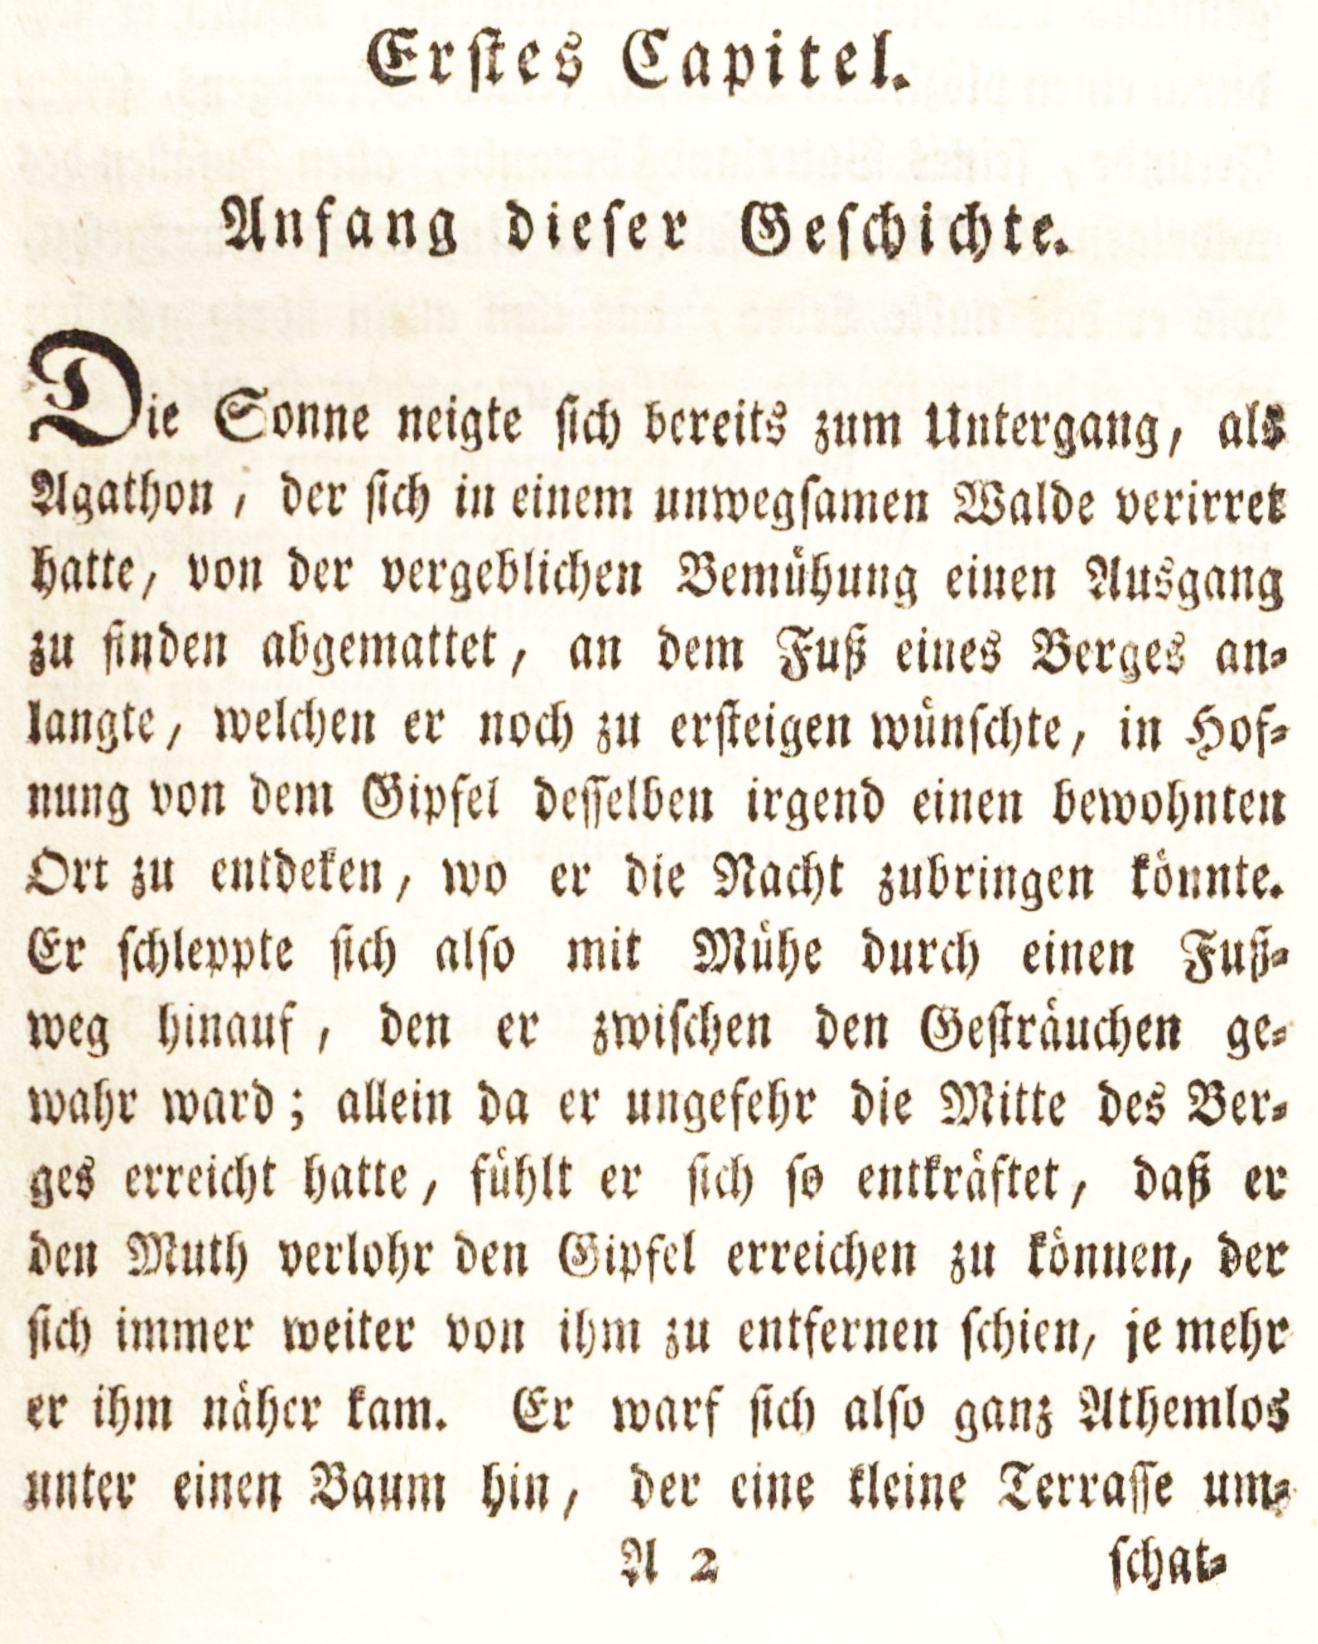
\includegraphics[width=0.45\textwidth]{\GRAPHPATH/agathon1e}\\[0.5\baselineskip]
  {\tiny Wieland, Christoph Martin: Geschichte des Agathon. Bd.\ 1. Frankfurt (Main) u.\,a., 1766. In: Deutsches Textarchiv\\[-1\baselineskip]
    \url{http://www.deutschestextarchiv.de/wieland_agathon01_1766>}}
\end{frame}

\begin{frame}
  {Die Entwicklung von Schreibprinzipien}
  \centering
  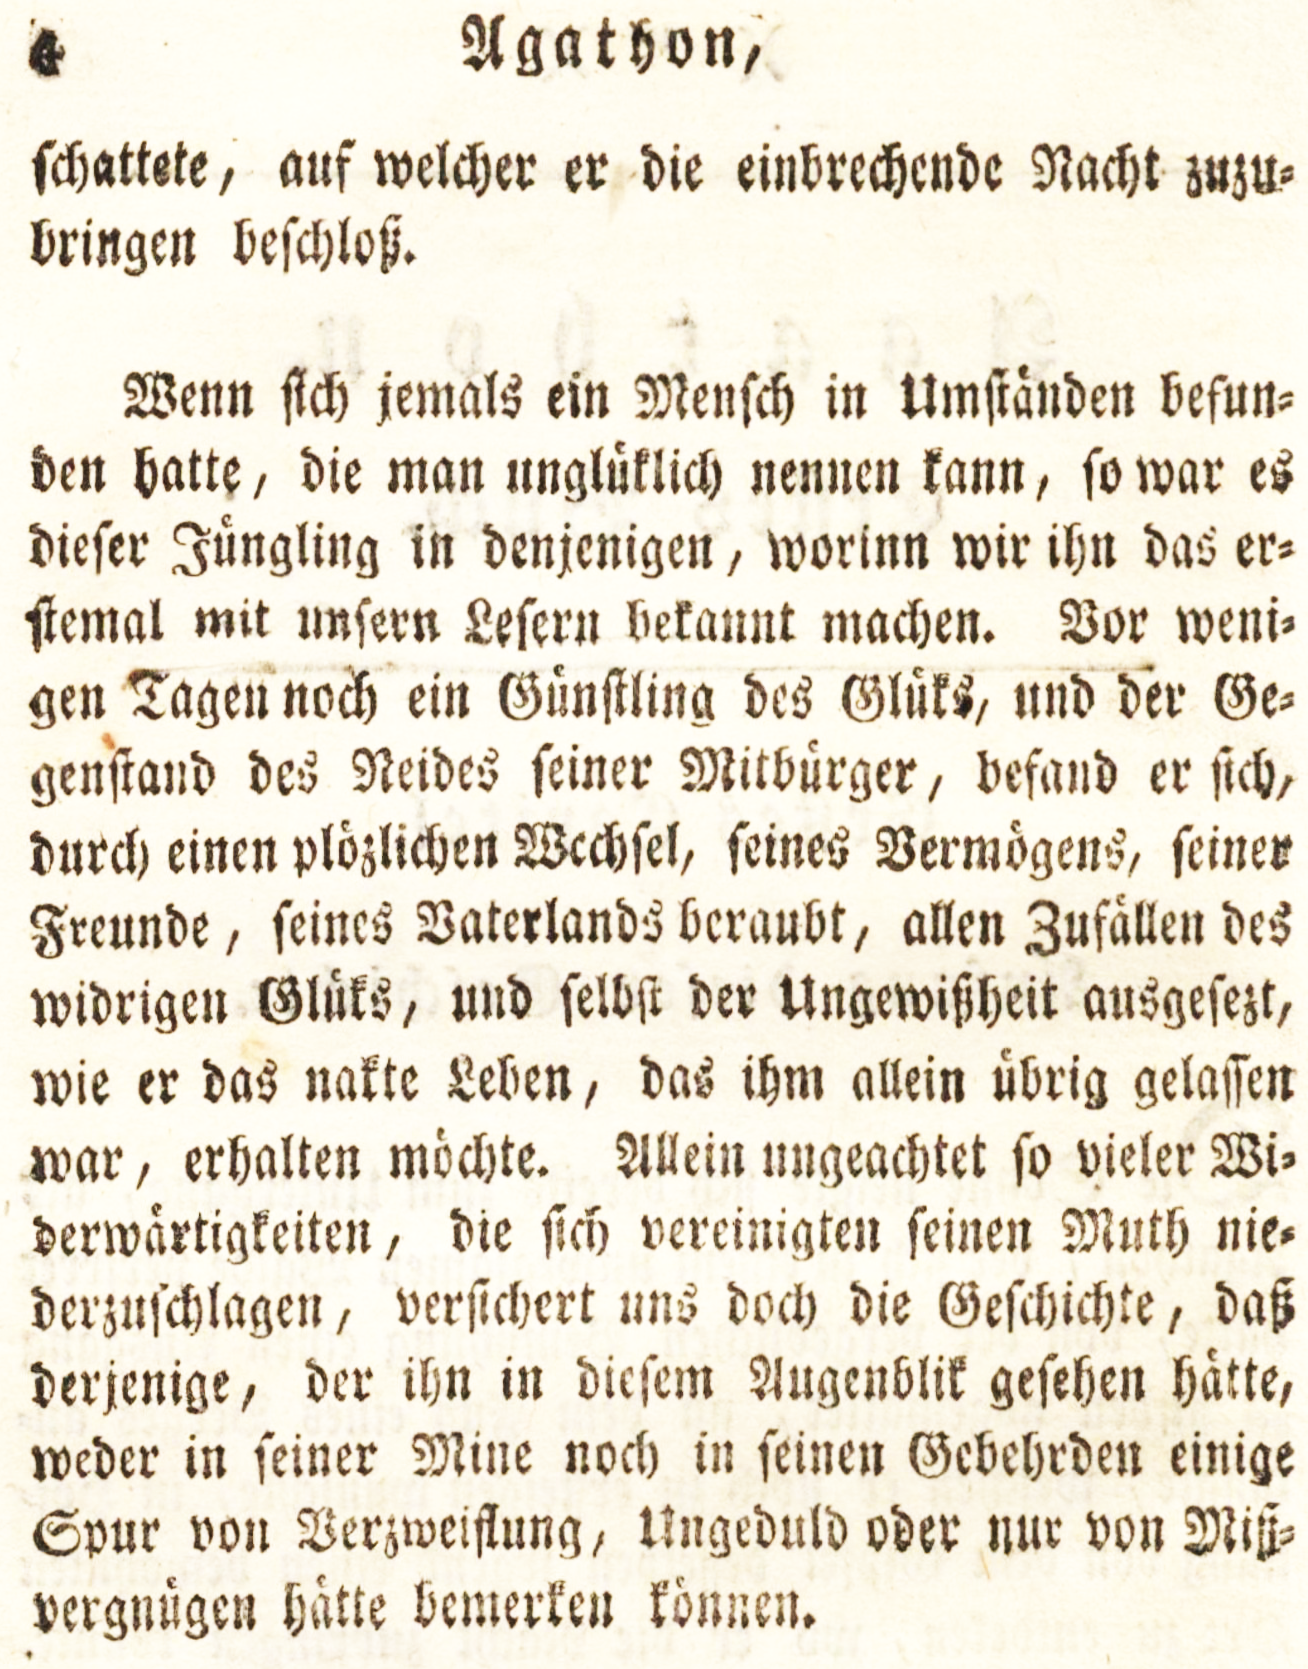
\includegraphics[width=0.45\textwidth]{\GRAPHPATH/agathon2e}\\[0.5\baselineskip]
  {\tiny Wieland, Christoph Martin: Geschichte des Agathon. Bd.\ 1. Frankfurt (Main) u.\,a., 1766. In: Deutsches Textarchiv\\[-1\baselineskip]
    \url{http://www.deutschestextarchiv.de/wieland_agathon01_1766>}}
\end{frame}

\begin{frame}
  {Zur Erinnerung: unerklärte Doppelkonsonanten}
  \pause
  \centering
  \resizebox{0.85\textwidth}{!}{
    \begin{tabular}{lllllllll}
      \toprule
      & & & \textbf{ɪ} & \textbf{ʊ} & \multicolumn{2}{l}{\LocStrutGrph\textbf{ɛ̆}} & \textbf{ɔ} & \textbf{ă} \\
      \midrule

      \multirow{4}{*}{\rotatebox{90}{\textbf{ungespannt}}}

      & \multirow{2}{*}{\rotatebox{90}{\textbf{offen}}}
      & \textbf{einsilb.}  & \textit{\Nono}  & \textit{\Nono}           & \multicolumn{2}{l}{\LocStrutGrph\textit{\Nono}}         & \textit{\Nono}        & \textit{\Nono}           \\
      && \textbf{zweisilb.}  & \textit{Li.\alert{pp}e} & \textit{Fu.\alert{tt}er}         & \multicolumn{2}{l}{\LocStrutGrph\textit{We.\alert{ck}e}}        & \textit{o.\alert{ff}en}       & \textit{wa.\alert{ck}er}         \\
        & \multirow{2}{*}{\rotatebox{90}{\textbf{gesch.}}}
        & \textbf{einsilb.}  & \textit{Ki\rot{nn}}   & \textit{Schu\rot{tt}}    & \multicolumn{2}{l}{\LocStrutGrph\textit{Be\rot{tt}}}           & \textit{Ro\rot{ck}}         & \textit{Wa\rot{tt}}            \\
        && \textbf{zweisilb.}  & \textit{Rin.de} & \textit{Wun.der}        & \multicolumn{2}{l}{\LocStrutGrph\textit{Wen.de}}        & \textit{pol.ter}      & \textit{Tan.te}          \\

      \midrule

      \multirow{4}{*}{\rotatebox{90}{\textbf{gespannt}}}

      & \multirow{2}{*}{\rotatebox{90}{\textbf{offen}}}
        & \textbf{einsilb.}  & \textit{Knie}   & \textit{Schuh}       & \textit{Schnee, Reh}  & \textit{zäh}          & \textit{roh}          & (\textit{da})            \\
      && \textbf{zweisilb.}  & \textit{Bie.ne} & \textit{Kuh.le, Schu.le} & \textit{we.nig}       & \textit{Äh.re, rä.kel} & \textit{oh.ne, O.fen} & \textit{Fah.ne, Spa.ten} \\

      & \multirow{2}{*}{\rotatebox{90}{\textbf{gesch.}}}
        & \textbf{einsilb.}  & \textit{lieb}  & \textit{Ruhm, Glut}      & \textit{Weg}          & \textit{spät}           & \textit{rot}          & \textit{Tat}             \\
      && \textbf{zweisilb.}  & (\textit{lieb.lich}) & (\textit{lug.te})   & (\textit{red.lich})   & (\textit{wähl.te})     & (\textit{brot.los})   & (\textit{rat.los})       \\

      \midrule
      & & & \textbf{i} & \textbf{u} & \textbf{e} & \textbf{ε} & \textbf{o} & \textbf{a} \\

      \bottomrule
    \end{tabular}
  }\\
  \pause
  \Viertelzeile
  \raggedright
  \begin{itemize}[<+->]
    \item Warum \textit{Kinn}, \textit{Schutt}, \textit{Bett}, \textit{Rock}, \textit{Wattes}?
    \item \alert{nicht unterlassbare Gelenkschreibungen}
      \begin{itemize}[<+->]
        \item \textit{die Ki\alert{nn}e}
        \item \textit{des Schu\alert{tt}es}
        \item \textit{die Be\alert{tt}en}
        \item \textit{die Rö\alert{ck}e}
      \end{itemize}
    \item \alert{Die Schreibungen eines Stamms einander angleichen!} Sonst:
      \begin{itemize}[<+->]
        \item \textit{*Kin --- Kinne}
        \item \textit{Schut --- Schutt}
        \item \textit{Bet --- Betten}
        \item \textit{Rok --- Röcke}
      \end{itemize}
  \end{itemize}
\end{frame}

\begin{frame}
  {Andere Konstantschreibungen}
  \pause
  \begin{itemize}[<+->]
    \item andere Wortklassen
      \begin{itemize}[<+->]
        \item \textit{*plat --- pla\rot{tt} --- pla\alert{tt}er}
        \item \textit{*as --- a\rot{ß} --- a\alert{ß}en}
        \item aber: \textit{las --- lasen}
        \item \textit{*schlizte --- schli\rot{tz}te --- schli\alert{tz}en}
      \end{itemize}
      \Halbzeile
    \item andere Phänomene (nicht Silbengelenk oder \textit{ß})
      \begin{itemize}[<+->]
        \item \textit{*gest --- ge\rot{h}st --- ge\alert{h}en}
        \item \textit{*siest --- sie\rot{h}st --- se\alert{h}en}
        \item \textit{*Reume --- R\rot{äu}me --- R\alert{au}m}
        \item \textit{*leuft --- l\rot{äu}ft --- l\alert{au}fen}
      \end{itemize}
  \end{itemize}
\end{frame}

\section{Schreibprinzipien}

\begin{frame}
  {Zusammenfassung der besprochenen Schreibprinzipien I}
  \pause
  Korrespondenzen zur Phonologie\\
  \Zeile
  \pause
  \begin{itemize}[<+->]
    \item \alert{phonologisches Schreibprinzip}
      \begin{itemize}[<+->]
        \item Konsonantenzeichen (inkl.\ Di- und Trigraphen)\\
          entsprechen 1:1 zugrundeliegenden Segmenten.
        \item Paare von zugrundeliegendem gespanntem und ungespanntem Vokal\\
          entsprechen jeweils nur einem Vokalzeichen 
      \end{itemize}
     \Zeile 
    \item \alert{Prinzip der Silbengelenkschreibung}
      \begin{itemize}[<+->]
        \item Silbengelenke werden durch Konsonantendopplung markiert.
        \item Für Di- und Trigraphen gilt dies nicht.
      \end{itemize}
  \end{itemize}
\end{frame}

\begin{frame}
  {Zusammenfassung der besprochenen Schreibprinzipien II}
  Korrespondenzen zur Morphosyntax\\
  \Zeile
  \pause
  \begin{itemize}[<+->]
    \item \alert{Prinzip der Konstantschreibung}
      \begin{itemize}[<+->]
        \item Die Formen eines lexikalischen Wortes werden so ähnlich geschrieben,\\
          wie es angesichts der anderen Prinzipien möglich ist.
      \end{itemize}
      \Zeile
    \item \alert{Prinzip der Spatienschreibung}
      \begin{itemize}[<+->]
        \item Syntaktische Wörter werden durch Spatium getrennt.
        \item \grau{Zweifelsfälle dabei sind morphosyntaktisch, nicht graphematisch.}
      \end{itemize}
      \Zeile
    \item \alert{Prinzip der positionsunabhängige Majuskelschreibung}
      \begin{itemize}[<+->]
        \item Substantive werden positionsunabhängig\\
          mit einleitender Majuskel geschrieben.
      \end{itemize}
  \end{itemize}
\end{frame}

\begin{frame}
  {Das wars!}
  \pause
  \begin{itemize}[<+->]
    \item Das war der Stoff der VL dieses Semesters.
    \item \alert{Vielen Dank fürs Zuhören und Fragenstellen!}
    \item Trotz der Arbeitsbelastung hat mir diese die Lehrveranstaltung\\
      den meisten Spaß in meiner gesamten Zeit als Dozent*in gemacht.
      \Zeile
    \item Jetzt kommt noch zweimal "`ernste Worte"'.
    \item Die Folien enthalten viel Text (ganze Sätze!), weil Sie das\\
      sonst nirgendwo nachlesen können.
      \Halbzeile
    \item Dann endlich die Klausurbesprechung!
  \end{itemize}
\end{frame}

\section{Alles falsch?}

\begin{frame}
  {Nochmal zur Grammatik in der Schule}
  \pause
  Wie ich höre\ldots
  \pause
  \begin{itemize}[<+->]
    \item \rot{Frustration} darüber, was alles \textit{falsch} sein soll
    \item insbesondere (angeblich) in Schulbüchern
      \Halbzeile
    \item außerdem: \alert{Es funktioniert doch!}
  \end{itemize}
\end{frame}
  
  
  
\begin{frame}
  {Deutschunterricht}
  \pause
  \alert{Worum geht es in der Schule beim Deutschunterricht nochmal?}\\
  \Halbzeile
  \pause
  \begin{itemize}[<+->]
    \item Erwerb von Schrift (= Zeichen) und Schreibung (= Prinzipien)
    \item Erwerb der \alert{Schriftsprache} (= \alert{völlig neue Grammatik})
    \item Erwerb der \alert{überregionalen Standardsprache} (= neue Grammatik)
    \item Erwerb der \alert{Bildungssprache} (basiert stark auf Schriftsprache)
      \begin{itemize}[<+->]
        \item komplexe Sachverhalte
        \item argumentative Strukturen
        \item Registersensitivität
        \item Variantenbewusstsein, \ldots
        \item \alert{und die zugehörigen sprachlichen Formen}
      \end{itemize}
      \Halbzeile
    \item Ist Deutsch eigentlich ein ungewöhnliches Schulfach?
  \end{itemize}
\end{frame}

\begin{frame}
  {Möglichkeit A: das Wissen an sich}
  \pause
  \begin{itemize}[<+->]
    \item \alert{Schulfächer lehren selbstbewusst ihre \alert{Inhalte}:}
      \begin{itemize}[<+->]
        \item Biologie: Ranviersche Schnürringe, Natrium-Kalium-Pumpe, \ldots
        \item Geschichte: Schlacht von Worringen, Hanse, Völkerwanderung, \ldots
        \item Erdkunde: Löss-Böden, Schwemmland, Kontinentaldrift, \ldots
        \item Physik: idealisierte Wagen auf idealisierten schiefen Ebenen,\\
          Gravitationsgesetze, Ohmsches Gesetz, \ldots
        \item Chemie: Wasserstoffbrückenbindungen, Schalenmodell, Veresterung, \ldots
        \item Mathematik: Ableiten und Integrieren, Vektor- und Matrizenrechnung, \ldots
      \end{itemize}
      \Viertelzeile
    \item Das ist Wissen darum, wie die Welt funktioniert.
    \item Es gibt ein Verständnis für die westlich-wissenschaftliche Weltsicht.
    \item \rot{Was davon erwarten Sie, im Leben praktisch zu brauchen?}
  \end{itemize}
\end{frame}

\begin{frame}
  {Und das Schulfach Deutsch?}
  \pause
    \begin{itemize}[<+->]
      \item Erwerbsaufgaben (\rot{keine} Wissensvermittlung): Das muss ja sein. 
      \item Literatur: recht selbstbewusst (\zB wichtige Werke der dt.\ Literatur)
        \Halbzeile
      \item Wissen darum, wie Sprache funktioniert: \rot{Oh Gott! Nein! Das hat ja\\
        gar keinen praktischen Nutzen (jenseits der Erwerbsaufgaben)!}
    \end{itemize}
\end{frame}

\begin{frame}
  {Das Problem mit Wissen an sich: die Genauigkeit!}
  \pause
  \begin{itemize}[<+->]
    \item Angenommen, es würden grammatische\slash linguistische Inhalte\\
      als Fachwissen an Schulen gelehrt\ldots
    \item \alert{Dann müsste es aber sachlich korrekt sein bzw.\\
      dem Forschungsstand entsprechen!}
      \Halbzeile
    \item \rot{Das, was in Grammatik unterrichtet wird, entspricht\\
      auf jeden Fall nicht dem Forschungsstand.}
      \Zeile
    \item Es lassen sich de facto seit 50 Jahren kaum Änderungen\\
      am Schulstoff politisch durchsetzen.
    \item Die Linguistik hat in den Siebzigern ihren Teil dazu beigetragen,\\
      dass es große Skepsis ihr gegenüber (als Fachdisziplin) gibt.
    \item Man wollte Chomskys "`Generative Transformationsgrammatik"'\\
      an die Schulen bringen.
    \item \raisebox{-.2\height}{
\includegraphics[width=1.25em]{\GRAPHPATH/emoji_mourning}}
  \end{itemize}
\end{frame}

\begin{frame}
  {Möglichkeit B: vor allem die Erwerbsaufgaben}
  \pause
  \begin{itemize}[<+->]
    \item Das entspricht dem Ist-Zustand.
    \item Meinethalben kann das so bleiben.
      \Halbzeile
    \item Was ist dann wichtig?
      \begin{itemize}[<+->]
        \item \alert{Sprachbetrachtung} (= Reflexion über Form und Funktion)
        \item unmöglich exhaustiv unterrichtbar, also \alert{Methodenvermittlung}
        \item für deklarativen Kern: \alert{widerspruchsfrei, dem Phänomen angemessen}
      \end{itemize}
  \end{itemize}
\end{frame}


\begin{frame}
  {Anforderungen bei Möglichkeit B}
  \pause
    \begin{itemize}[<+->]
      \item \alert{Form und Funktion der eigenen Sprache verstehen}
      \item selber in der Lage sein, \alert{Generalisierungen zu erarbeiten}
      \item zum Phänomen \alert{das passende Material zusammenstellen}
      \item \alert{Operationalisierungen} erarbeiten und Schüler*innen anbieten
        \Halbzeile
      \item \rot{Erkennen und Einstufen von Erwerbsproblemen}
        \Halbzeile
      \item \rot{fair und begründet bewerten}
        \Halbzeile
      \item \rot{Die Didaktisierung kann nicht darin bestehen, den Schüler*innen\\
        Material und Methoden anzubieten, aus denen die entsprechenden\\
      Kompetenzen prinzipiell nicht erwerbbar sind.}
      \Halbzeile
    \item Beispiel: die \textit{Wie}-Wörter
      \begin{itemize}[<+->]
        \item \textit{der rote Trecker}
        \item \textit{Wie ist der Trecker?} --- \alert{(\textit{Der Trecker ist}) \textit{rot.}}
        \item \grau{Die Antwort ist immer ein Kopulsatz.}
      \end{itemize}
  \end{itemize}
\end{frame}

\begin{frame}
  {Ein Beispiel: Adjektive als Wie-Wörter}
  \begin{itemize}[<+->]
    \item OK für bestimmte \alert{qualitative Adjektive}
      \Halbzeile
    \item viele Adjektivklassen sind aber keine Wie-Wörter:
      \begin{itemize}[<+->]
        \item \rot{temporal}: der \rot{gestrige} Vorfall
        \item \rot{quantifizierend} (relativ, Zählsubstantiv): \textit{die \rot{zahlreichen} Äpfel}
        \item \rot{quantifizierend} (relativ, Stoffsubstantiv): \textit{\rot{reichlich} Apfelmus}
        \item \rot{quantifizierend} (absolut): \textit{die \rot{drei} Bienen}
        \item \rot{intensional}: \textit{der \rot{ehemalige} Präsident}\slash\textit{die \rot{fiktive} Gestalt}
        \item \rot{phorisch}: \textit{die \rot{obigen}}/\textit{\rot{weiteren}}/\textit{\rot{anderen} Ausführungen}
        \item \rot{qualitativ-relativ} (sortensensitiv): \textit{eine \rot{schnelle} Schnecke}
      \end{itemize}
      \Halbzeile
    \item Fällt Ihnen was auf?
      \begin{itemize}[<+->]
        \item Das sind im Wesentlichen die, die nicht prädikativ verwendbar sind.
        \item Ach, basiert der Test also vielleicht einfach darauf?
        \item Aber viele Adjektive sind doch gar nicht prädikativ verwendbar.
          \Halbzeile
        \item[ ] \raisebox{-0.5\height}{
\includegraphics[height=4em]{\GRAPHPATH/doh}}
      \end{itemize}
  \end{itemize}
\end{frame}

\begin{frame}
  {Inhaltliche Stolperfallen}
  \pause
  \begin{itemize}[<+->]
    \item linguistisch eine klare Angelegenheit:
      \begin{itemize}[<+->]
        \item \rot{Die Kategorie \textit{Adjektiv} kann man nicht über "`wie"' erfragen!}
        \item im Prinzip nur die Subklasse der prädikativ verwendbaren Adjektive
      \end{itemize}
     \Halbzeile
    \item inhaltliche Gefahr
      \begin{itemize}[<+->]
        \item Wenn Sie Kinder dressieren, \rot{alle} Klassen mit "`wie"' zu erfragen\ldots
        \item \ldots dann \rot{zerstören Sie die wahrscheinlich bereits existierende semantische Intuition}, die das Kind hat.
          \Halbzeile
        \item \rot{Totalschaden in Vermittlung von Bildungssprache\slash Sprachbetrachtung}
      \end{itemize}
  \end{itemize}
\end{frame}

\begin{frame}
  {Didaktische Stolperfallen}
  \pause
  \begin{itemize}[<+->]
    \item didaktische Gefahr
      \begin{itemize}[<+->]
        \item "`Die Kinder können es doch gut mit der Wie-Frage!"' (s. nächste Folie)
      \end{itemize}
      \Halbzeile
    \item Fragen Sie immer:
      \Halbzeile
      \begin{itemize}[<+->]
        \item Ist das, was ich unterrichte (vor-)wissenschaftliches Wissen an sich \alert{und gibt präzise linguistische Generalisierungen wieder?} --- \gruen{OK!}
          \Halbzeile
        \item Oder trägt es zur Sprach(betrachtungs)kompetenz de*r Schüler*innen bei, indem sie durch die Übung \alert{Kompetenzen} erwerben, die zur \alert{besseren Beherrschung sprachlicher Mittel} (i.\,w.\,S.) führen? --- \gruen{OK!}
          \Halbzeile
        \item Keins von beidem? --- \rot{Nicht OK!} Dann lassen Sie es lieber.
      \end{itemize}
  \end{itemize}
\end{frame}

\begin{frame}
  {Eine Aufgabe zu Adjektiven I}
  \pause
  Warum können die Kinder das so gut mit der Wie-Frage?\\
  \Halbzeile
  \pause
  \centering
  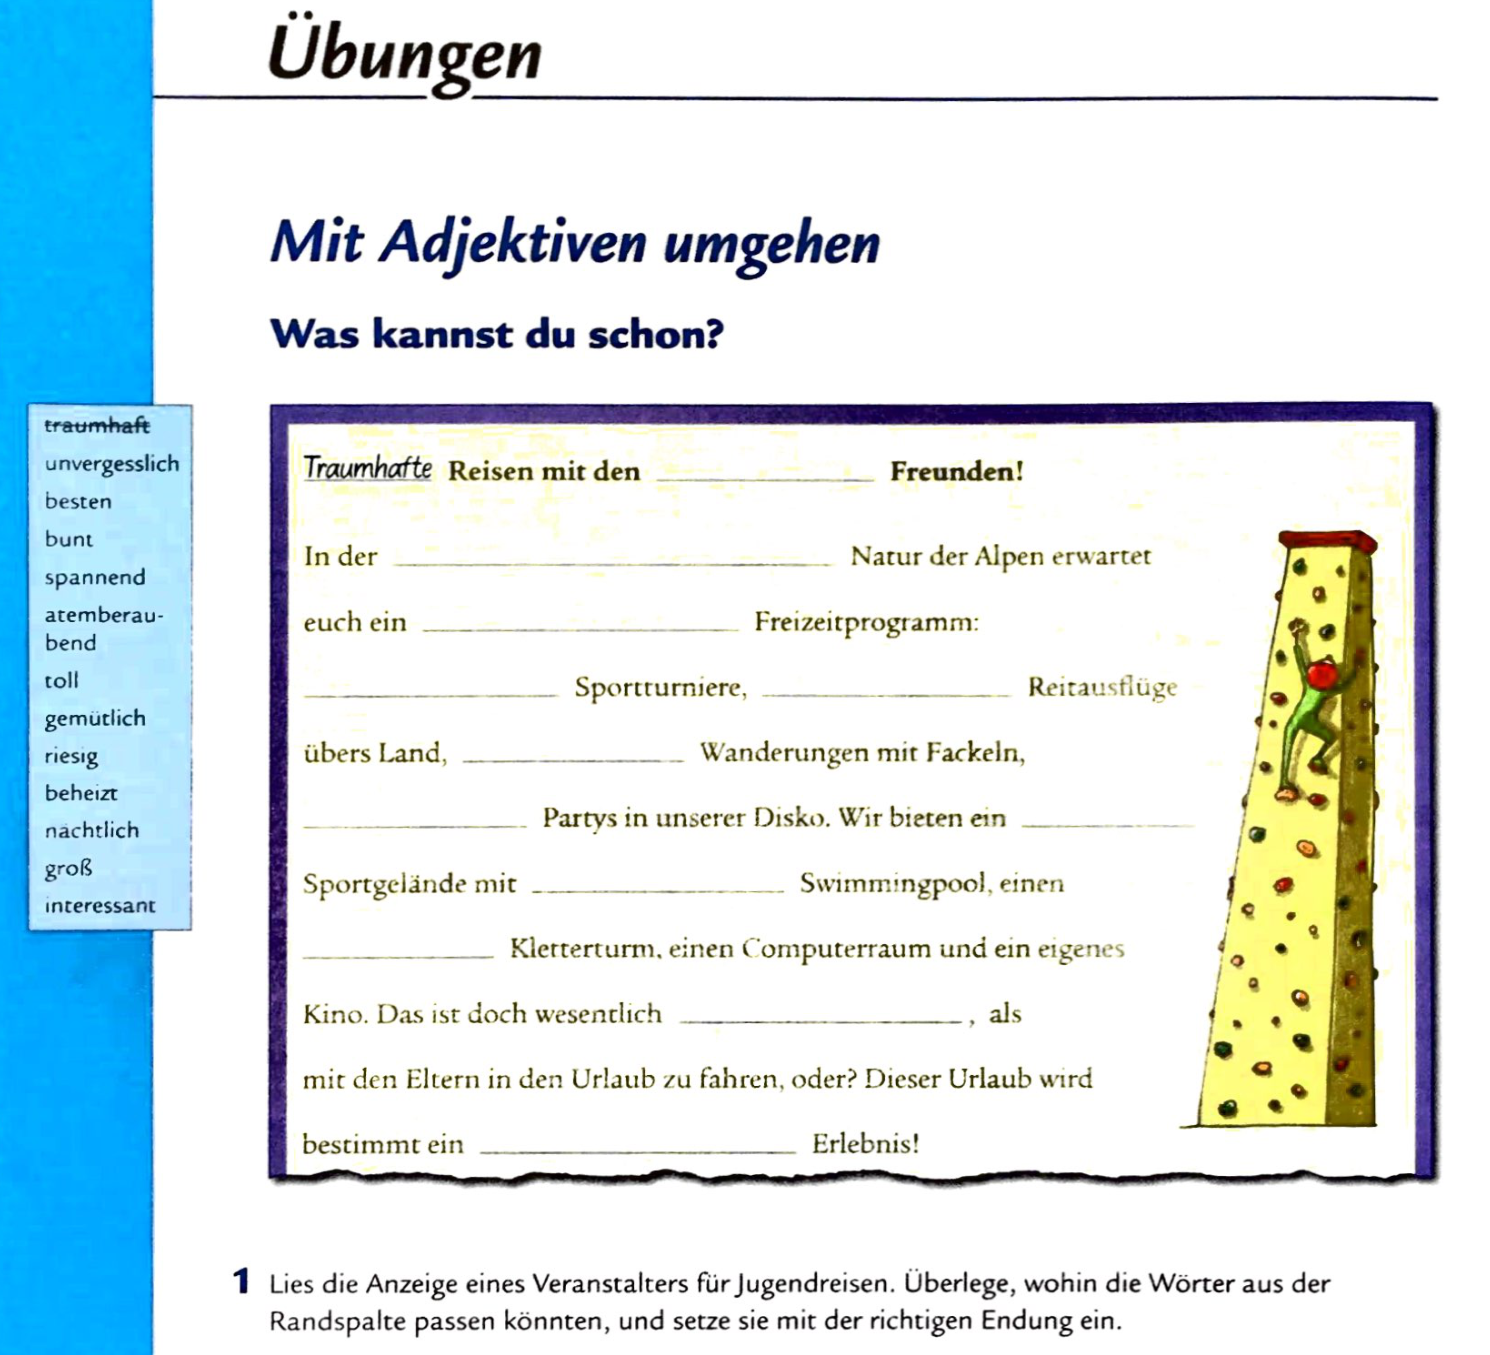
\includegraphics[width=0.65\textwidth]{\GRAPHPATH/adjektive1}
\end{frame}

\begin{frame}
  {Eine Aufgabe zu Adjektiven II}
  Gut! Bezug zur Funktion sprachlicher Mittel. Aber\ldots\\
  \Zeile
  \pause
  \centering
  
\includegraphics[width=0.7\textwidth]{\GRAPHPATH/adjektive2}
\end{frame}

\section{Meine Meinung zu sprachlicher Toleranz}

\begin{frame}
  {Das tut ja weh!}
  \pause
  Angeblich wurden folgende Sätze als schmerzhaft (sic!) falsch empfunden.
  \pause
  \Viertelzeile
  \begin{exe}
    \ex \rot{Es friert mich}.
    \pause
    \ex Die Mechanikerin \rot{bekommt} von der Auszubildenden \rot{geholfen}.
    \pause
    \ex Die Erklärung \rot{macht Sinn}.
    \pause
    \ex \rot{Gebe} deiner Schwester jetzt das Buch.
  \end{exe}
  \pause
  \begin{itemize}[<+->]
    \item Das ist die bildungssprachliche Verwendung von \textit{frieren}! (Duden 1)
    \item \alert{Rezipientenpassiv ist auch geschrieben Standard} (Duden 4, §807–810).
      \begin{itemize}[<+->]
        \item Meist "`akzeptabler"' mit Akkusativ:\\
          \textit{Elena bekam von der Trainerin die Sprungtechnik erklärt.}
        \item partiell \alert{regionale Variation} (\textit{erhalten}, \textit{bekommen}, \textit{kriegen})
      \end{itemize}
    \item \textit{Sinn machen} kommt nicht aus dem Englischen und ist uralt.
    \item \alert{Der normalisierte Imperativ der vierstufigen Verben ist regional üblich},\\
      wird aber in der Tat im Standard nicht empfohlen (Duden 4, §609)
    \item \rot{Auf jeden Fall geht es um die alltägliche Sprache Ihrer Mitmenschen!}
  \end{itemize}
\end{frame}

\begin{frame}
  {Standard und andere Varietäten}
  \pause
  \begin{itemize}[<+->]
    \item Standard ist ein \alert{Kompromiss}, ein \alert{Versuch} den kleinsten gemeinsamen \alert{überregionalen und nicht soziolektal geprägten sprachlichen} Nenner zu beschreiben.
    \item hat nichts mit \rot{alt} oder \rot{ursprünglich} zu tun, wird \alert{ständig angepasst}
      \Halbzeile
    \item \alert{Lehrer*innen sind für die Vermittlung des Standards zuständig.}
    \item \rot{Aber was erlaubt es irgendwem, die Sprache anderer\\
      als schmerzhaft oder ekelhaft zu bezeichnen?}
  \end{itemize}
\end{frame}

\begin{frame}
  {Die Provokationsfolie}
  \pause
  \begin{itemize}[<+->]
    \item Wie finden Sie das?
      \Halbzeile
      \begin{itemize}[<+->]
        \item "`Häng dir was vors Gesicht. Deine Augen sind ekelhaft."'
          \Viertelzeile
        \item Bei deiner Figur sieht das Hemd echt widerlich aus.
          \Viertelzeile
        \item "`Die Schwulen sollen doch woanders hingehen. Ich muss kotzen."'
          \Viertelzeile
        \item Sag nicht nochmal "`Sie bekommt geholfen."' Das tut ja weh.
          \Viertelzeile
        \item Wir verkaufen nur an Weiße\slash Arier\slash\ldots.
          \Viertelzeile
        \item "`Roberto Blanco war immer ein wunderbarer Neger."'
          \Viertelzeile
        \item Der sagt "`isch"' statt "`ich"'. Wir stellen wohl lieber jemanden ein,\\
          der richtiges Deutsch kann.
      \end{itemize}
      \Zeile
    \item Unterschied: \rot{Grad der Explizitheit\slash Implizitheit der Diskriminierung}
  \end{itemize}
\end{frame}


\begin{frame}
  {Diskriminierung, offen oder versteckt?}
  \pause
  \begin{itemize}[<+->]
    \item Implizite Diskriminierung (\zB gegenüber Migrant*innen,\\
      LGBTQ-Personen) ist unser Hauptproblem "`in Diskriminierung"'.
    \item \rot{Erfahrungsgemäß kann implizite Diskriminierung\\
      jederzeit explizit werden.}
      \Halbzeile
    \item Implizit heißt eben auch \alert{unbewusst}. Das ist schnell passiert.
      \Halbzeile
    \item Ich nehme mich überhaupt nicht aus und sehe mich als Lernende*.
    \Halbzeile
  \end{itemize}
\end{frame}

\begin{frame}
  {Standard\slash Dialekt\slash Soziolekt in der Schule}
  \pause
  \begin{itemize}[<+->]
    \item \rot{auf keinen Fall sprachliche Diskriminierung}
    \item im Gegenteil: \alert{Dia- und Soziolekte erhalten}
    \item Standard \alert{bewusst als neue zusätzliche Varietät} unterrichten,\\
      die genau definierte\alert{Anwendungskontexte} hat\\
      (= Variantenbewusstsein)
      \Halbzeile
    \item nicht unselektiv\slash pauschal "`richtig"' gegen "`falsch"' stellen
    \item vor allem \rot{niemals nach "`Geschmacksurteilen"' bewerten},\\
      denn \rot{Lehrer*innen korrigieren oft inkonsistent} und\\
      streichen viel mehr als falsch an, als wirklich normativ falsch ist\\
      (\citealt[4--7]{Eisenberg2004}, \citealt[319--324]{Haecker2009})
      \Halbzeile
    \item \alert{Wenn Sie es nicht genau wissen, schauen Sie es nach!}
    \item \ldots oder diskutieren Sie das Phänomen im Rahmen des Systems.
  \end{itemize}
\end{frame}


\section{Vorschau}

\begin{frame}
  {Was heißt Klausurvorbereitung?}
  \pause
  \begin{itemize}[<+->]
    \item inhaltliche Fragen?
    \item Fragen zur Probeklausur?
    \item ansonsten meine vorbereiteten Übungen
  \end{itemize}
  \pause
  \Halbzeile
  \begin{center}
    Bitte lesen Sie bis nächste Woche:\\
    \alert{Nichts. Oder das ganze Buch nochmal.}
  \end{center}
\end{frame}

\begin{frame}
  {Klausurtipps}
  \pause
  \alert{Rechnen Sie mit:}
  \Halbzeile
  \pause
  \begin{itemize}
    \item<4> Anwendung von grammatischem Wissen auf Beispiele
    \item<5> Aufgaben, bei denen die Prämisse verneint werden muss
    \item<6> Aufgaben, bei denen ich Ihnen mehr gebe als nötig
    \item<7> Aufgaben, die "`anders herum"' gestellt sind
    \item<8> Aufgaben, bei denen Sie nicht komplette Analysen erstellen,\\
      sondern schnell bestimmte Eckpunkte finden müssen
    \item<9> kurz gesagt: Aufgaben wie im echten grammatischen Leben
  \end{itemize}
  \pause
  \pause
  \pause
  \pause
  \pause
\end{frame}

